% 2.2.PrepareLibrary.tex
%	Last update: 2019/07/24 F.Kanehori
%newpage
\subsection{K11cOJIYzUE65BBo}
\label{subsec:PrepareLibrary}

\noindent
\KLUDGE ダウンロードが済んだら\SprTop{/core/src}\KLUDGE に移動してください。

\noindent
\KLUDGE まず、配布されたファイル\CMakeLists{.Lib.dist}\KLUDGE を
\CMakeLists{}\KLUDGE という名前でコピーします
(\KLUDGE 誤コミットを防止するためにもリネームではなくコピーしてください)。

\medskip
\ifLwarp
	\begin{figure}[h]
	    \begin{center}
	    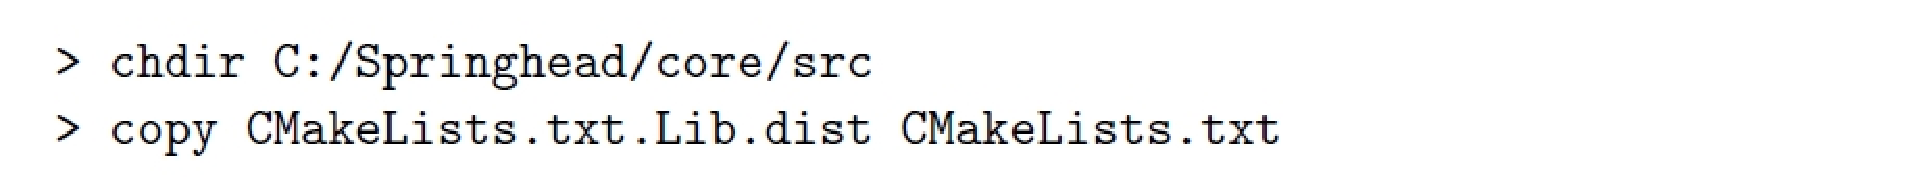
\includegraphics[width=\textwidth]{fig/command-2-2-a.eps}
	    \end{center}
	    \label{fig:DownloadTree}
	\end{figure}
\else
\begin{narrow}[15pt]
	\CmndBox{%
		\textgreater  chdir C:/Springhead/core/src\\
		\textgreater  copy CMakeLists.txt.Lib.dist CMakeLists.txt
	}
\end{narrow}
\fi

\medskip
\noindent
\KLUDGE 自前でインストールしているパッケージ
(\tt{boost}, \tt{glew}, \tt{freeglut}, \tt{glui})\KLUDGE を使用する場合
\KLUDGE およびライブラリファイルとヘッダファイルのインストール先を指定する場合には、
\KLUDGE さらに、
\KLUDGE 配布されたファイル\CMakeConf{.dist}\KLUDGE を\CMakeConf{}\KLUDGE という名前でコピーして
\KLUDGE 必要な編集をします。
\KLUDGE 編集の方法については\CMakeConf{}\KLUDGE に記述されています
(``\tt{=ESCAPEx23=set(variable \it{value})}''\KLUDGE から``\tt{=ESCAPEx23=}''\KLUDGE を削除し、
``\it{value}''\KLUDGE を適切に設定し直す)\KLUDGE 。

\def\cite=ESCAPEx23=1{\hspace{10pt}\footnotesize{=ESCAPEx23=1}}
\def\somewhere{"C:/\it{somewhere}/\it{appropreate}"}
\medskip
\ifLwarp
	\begin{figure}[h]
	    \begin{center}
	    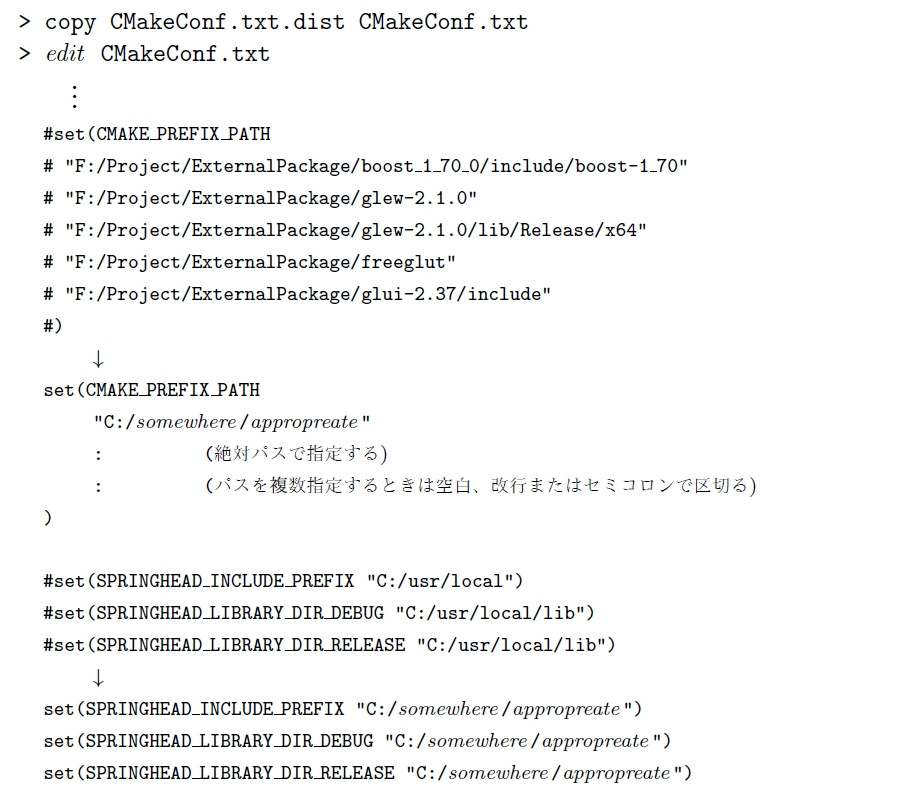
\includegraphics[width=\textwidth]{fig/command-2-2-b.eps}
	    \end{center}
	    \label{fig:DownloadTree}
	\end{figure}
\else
\begin{narrow}[15pt]
	\CmndBox{%
		\textgreater  copy CMakeConf.txt.dist CMakeConf.txt\\
		\textgreater  \it{edit} CMakeConf.txt\\
		\hspace{20pt}$\vdots$\\
	\cite{=ESCAPEx23=set(CMAKE\_PREFIX\_PATH}\\
	\cite{=ESCAPEx23= "F:/Project/ExternalPackage/boost\_1\_70\_0/include/boost-1\_70"}\\
	\cite{=ESCAPEx23= "F:/Project/ExternalPackage/glew-2.1.0"}\\
	\cite{=ESCAPEx23= "F:/Project/ExternalPackage/glew-2.1.0/lib/Release/x64"}\\
	\cite{=ESCAPEx23= "F:/Project/ExternalPackage/freeglut"}\\
	\cite{=ESCAPEx23= "F:/Project/ExternalPackage/glui-2.37/include"}\\
	\cite{=ESCAPEx23=)}\\
	\cite{\hspace{20pt}$\downarrow$}\\
	\cite{set(CMAKE\_PREFIX\_PATH}\\
	\cite{\hbox to 20pt{}\somewhere}\\
	\cite{\hspace{20pt}:\hspace{40pt}{(\rm{\KLUDGE 絶対パスで指定する)}}}\\
	\cite{\hspace{20pt}:\hspace{40pt}%
		{(\rm{\KLUDGE パスを複数指定するときは空白、改行またはセミコロンで区切る)}}}\\
	\cite{)}\\
	\cite{}\\
	\cite{=ESCAPEx23=set(SPRINGHEAD\_INCLUDE\_PREFIX       "C:/usr/local")}\\
	\cite{=ESCAPEx23=set(SPRINGHEAD\_LIBRARY\_DIR\_DEBUG   "C:/usr/local/lib")}\\
	\cite{=ESCAPEx23=set(SPRINGHEAD\_LIBRARY\_DIR\_RELEASE "C:/usr/local/lib")}\\
	\cite{\hspace{20pt}$\downarrow$}\\
	\cite{set(SPRINGHEAD\_INCLUDE\_PREFIX       \somewhere)}\\
	\cite{set(SPRINGHEAD\_LIBRARY\_DIR\_DEBUG   \somewhere)}\\
	\cite{set(SPRINGHEAD\_LIBRARY\_DIR\_RELEASE \somewhere)}
	}
\end{narrow}
\fi

\medskip
\noindent
\KLUDGE 以上で準備作業は終了です。

% end: 2.2.PrepareLibrary.tex
